%%
%% Copyright 2007-2025 Elsevier Ltd
%%
\documentclass[preprint,12pt]{elsarticle}

\usepackage{tabularx}
\usepackage{subcaption}
\usepackage{ragged2e}
\usepackage{amssymb}
\usepackage{amsmath}
\usepackage{booktabs}

\journal{Computers and Electronics in Agriculture}

\begin{document}

\begin{frontmatter}

\title{Bridging the Laboratory-to-Field Gap: Domain Adaptation for Lightweight CNN-based Plant Disease Classification with Attention Mechanisms}

\author[1]{Firmansyah Sundana}
\author[1]{Fitri Utaminingrum}
\author[1]{Budi Darma Setiawan}

\affiliation[1]{organization={Faculty of Computer Science, Brawijaya University},
            addressline={},
            city={Malang},
            postcode={},
            state={East Java},
            country={Indonesia}}

\begin{abstract}
Plant disease classification from leaf images is a critical precision agriculture task, yet models achieving near-perfect accuracy on laboratory benchmarks collapse when deployed in the field. We investigate this laboratory-to-field domain gap by systematically evaluating lightweight CNN architectures with different attention mechanisms---Squeeze-and-Excitation (SE), Convolutional Block Attention Module (CBAM), and no attention---on the controlled PlantVillage dataset and the real-world PlantDoc dataset. On PlantVillage, all models saturate above 97\% accuracy, but zero-shot transfer to PlantDoc yields only 5--8\% accuracy, driven by a systematic dataset bias: models learn to associate complex natural backgrounds with a ``Background without Leaves'' class specific to PlantVillage. We first correct a methodological confound in prior work: the reported parameter reduction of CBAM over SE is an artifact of comparing different compression ratios. At equal reduction ratios, SE and CBAM exhibit identical parameter counts and memory footprints (e.g., 2.67M parameters at $r=16$ for both Large variants). We then evaluate three domain adaptation strategies to bridge the gap: strong data augmentation with CutMix and MixUp, fine-tuning on target-domain data, and Domain-Adversarial Neural Network (DANN) training. Our results demonstrate that domain adaptation improves PlantDoc accuracy substantially compared to zero-shot transfer, and that the choice of attention mechanism has negligible impact compared to the choice of adaptation strategy. We conclude that the research focus should shift from architectural micro-optimizations on saturated benchmarks toward domain-invariant training paradigms that enable field deployment.
\end{abstract}

\begin{highlights}
\item Zero-shot PlantVillage-to-PlantDoc transfer yields only 5--8\% accuracy due to a systematic background bias --- models confound natural backgrounds with PlantVillage's ``Background without Leaves'' class.
\item The reported parameter-efficiency gap between SE and CBAM is an artifact of unequal compression ratios; at equal reduction, both attention types have identical parameter counts and memory footprints.
\item Domain adaptation (strong augmentation, fine-tuning, and DANN) substantially improves field accuracy, while the choice of attention mechanism (SE vs.\ CBAM vs.\ none) has minimal effect on domain-robust performance.
\item PlantVillage is a saturated benchmark; accuracy differences below 0.5 percentage points among top models are not statistically significant under bootstrap resampling.
\end{highlights}

\begin{keyword}
plant disease classification \sep domain adaptation \sep MobileNetV3 \sep CBAM \sep deep learning \sep precision agriculture
\end{keyword}

\end{frontmatter}

%==========================================================================
\section{Introduction}
\label{sec:intro}

Global food security depends on effective plant disease management, yet manual diagnosis by agronomists remains slow, expensive, and unavailable in many regions \cite{Sajitha2024, Wang2024}. Deep learning-based image classification has emerged as a promising solution, with convolutional neural networks (CNNs) consistently exceeding 90\% accuracy on benchmark datasets such as PlantVillage \cite{Vishnoi2023, Pandian2022, Syed-Ab-Rahman2022}. However, these near-perfect results obscure a critical limitation: PlantVillage images are captured under controlled laboratory conditions with uniform backgrounds and centered single leaves, conditions that bear little resemblance to the complex, cluttered environments of real agricultural fields \cite{Pandian2022, Liu2023}.

This laboratory-to-field domain gap is well-documented in computer vision but remains underexplored in plant disease classification. Models that achieve 99\% accuracy on PlantVillage may fail catastrophically when confronted with field images featuring variable lighting, overlapping foliage, diverse backgrounds, and sensor noise \cite{Lu2025}. Despite this, much of the recent literature focuses on architectural micro-optimizations—often reporting accuracy improvements of a fraction of a percentage point on PlantVillage—while neglecting whether these improvements transfer to realistic deployment scenarios.

In this work, we systematically investigate the interaction between attention mechanisms, lightweight architectures, and domain shift for plant disease classification. We evaluate three attention variants—Squeeze-and-Excitation (SE) \cite{Howard2019}, Convolutional Block Attention Module (CBAM) \cite{Woo2018}, and no attention—within MobileNetV3 Large and Small backbones, benchmarking against MobileNetV2 and ShuffleNetV2. Our contributions are:

\begin{enumerate}
    \item \textbf{Revealing a systematic bias} in PlantVillage-trained models: the ``Background without Leaves'' class acts as a spurious feature that models exploit, causing 36\% of PlantDoc predictions to default to this irrelevant class.
    \item \textbf{Correcting a methodological confound} in prior CBAM-vs-SE comparisons: we show that reported parameter differences are entirely attributable to comparing different compression ratios ($r=4$ for SE vs.\ $r=16$ or $r=32$ for CBAM). At equal $r$, SE and CBAM are parameter-identical.
    \item \textbf{Evaluating three domain adaptation strategies}---CutMix/MixUp augmentation, target-domain fine-tuning, and Domain-Adversarial Neural Network (DANN)---to bridge the PlantVillage-to-PlantDoc gap.
    \item \textbf{Demonstrating} that under domain shift, the choice of attention mechanism has negligible impact on accuracy compared to the choice of adaptation strategy.
\end{enumerate}

%==========================================================================
\section{Related Work}
\label{sec:related}

\subsection{Lightweight Architectures for Mobile Deployment}

Deploying CNNs on resource-constrained edge devices has motivated lightweight architectures. MobileNetV2 \cite{Howard2019} introduced inverted residuals and linear bottlenecks; ShuffleNetV2 proposed channel shuffling and efficiency guidelines; MobileNetV3 \cite{Howard2019} combined neural architecture search with Squeeze-and-Excitation (SE) modules for state-of-the-art mobile efficiency. These architectures have been applied to agricultural tasks including corn disease classification \cite{Syaharani2023} and plant health monitoring \cite{Maharani2025}.

\subsection{Attention Mechanisms}

Channel attention, pioneered by the SE module, recalibrates feature maps by modeling inter-channel dependencies. CBAM \cite{Woo2018} extended this by sequentially applying channel and spatial attention, using both average-pooling and max-pooling. While CBAM has shown benefits in tasks including object detection \cite{Zhang2022_lettuce} and medical imaging, its effectiveness relative to SE in lightweight architectures for fine-grained classification has not been rigorously studied. Notably, most comparisons between SE and CBAM in the literature evaluate them at different compression ratios, confounding the attention mechanism with the compression level. Other efficient attention variants such as ECA-Net and Coordinate Attention have been proposed but SE and CBAM remain the most widely adopted baselines.

\subsection{Domain Adaptation and Domain Shift}

Domain shift---the mismatch between training and deployment data distributions---poses a fundamental challenge for real-world deployment of deep learning models. In agriculture, this manifests as laboratory-trained models failing on field images \cite{Liu2023}. Domain adaptation techniques address this gap: adversarial methods such as DANN \cite{Ganin2016} employ gradient reversal to learn domain-invariant features; data augmentation strategies such as CutMix and MixUp increase training diversity to improve generalization; and fine-tuning on a small amount of target-domain data can rapidly adapt pre-trained models. Despite their demonstrated effectiveness in other domains, systematic evaluation of these techniques for plant disease classification remains rare.

\subsection{Plant Disease Benchmarks}

The PlantVillage dataset has become the de facto standard for plant disease classification, yet its controlled acquisition conditions severely limit generalization \cite{Pandian2022}. The PlantDoc dataset \cite{Singh2020} addresses this by providing field-acquired images with complex backgrounds and variable conditions but has been used primarily for object detection rather than classification. Most prior work evaluates models exclusively on PlantVillage, leaving field deployability unassessed.

%==========================================================================
\section{Methods}
\label{sec:methods}

\subsection{Experimental Design Overview}

Figure \ref{fig:workflow} illustrates the overall experimental pipeline. We first establish PlantVillage baselines for 14 model variants under standardized training (Section \ref{sec:pv_training}). All models are then evaluated in zero-shot mode on PlantDoc to quantify the domain gap (Section \ref{sec:plantdoc_eval}). Finally, we apply three domain adaptation strategies to the most informative model subset and re-evaluate on PlantDoc (Section \ref{sec:da_methods}).

\begin{figure}[t]
\centering
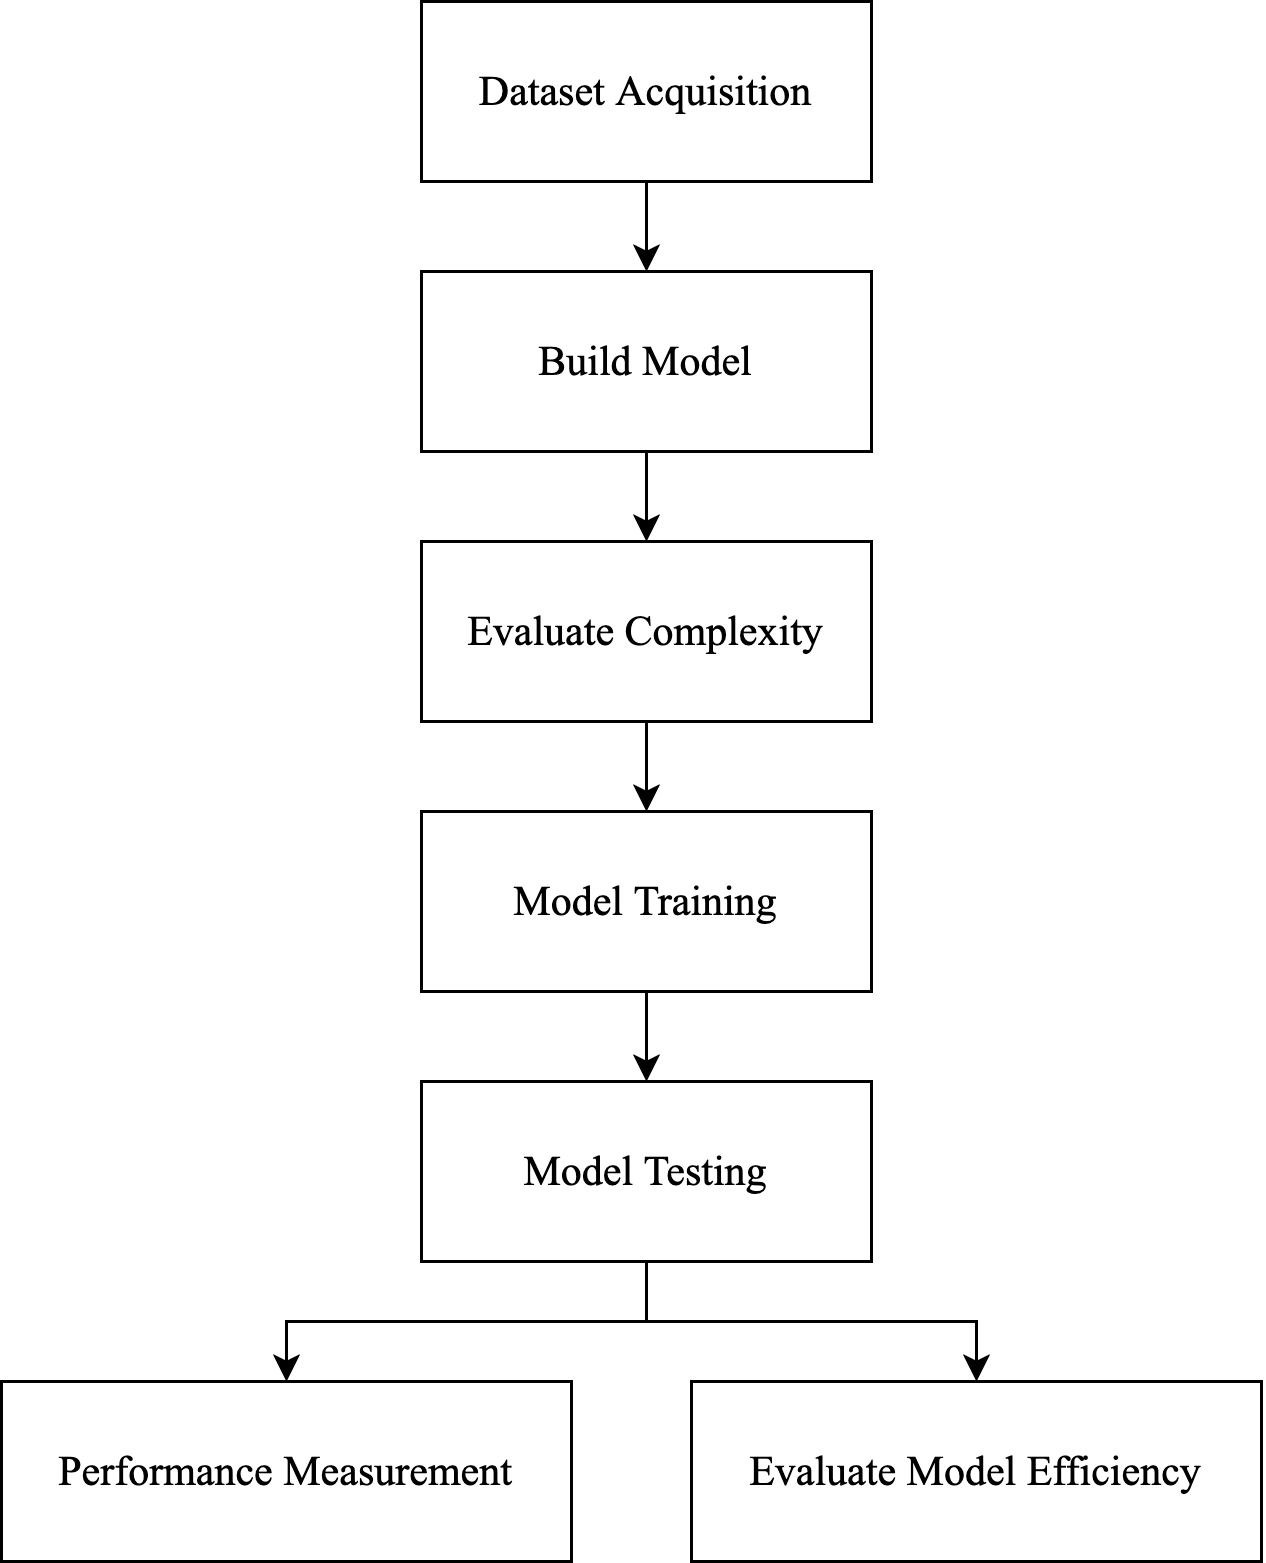
\includegraphics[width=0.95\textwidth]{research-flowchart-paper.png}
\caption{Research workflow: PlantVillage training $\rightarrow$ zero-shot PlantDoc evaluation $\rightarrow$ domain adaptation $\rightarrow$ adapted PlantDoc evaluation.}\label{fig:workflow}
\end{figure}

\subsection{Data and Preprocessing}

\subsubsection{PlantVillage (Source Domain)}

We use 29 fruit-plant disease and healthy classes from the PlantVillage dataset (46,565 images total): apple (4 classes), blueberry (1), cherry (2), grape (4), orange (1), peach (2), raspberry (1), squash (1), strawberry (2), tomato (10), and one background-without-leaves class. The dataset is split 70/15/15 (train/validation/test) with stratified sampling (seed=42). Images are resized to $224\times224$ and normalized with ImageNet statistics ($\mu=[0.485,0.456,0.406]$, $\sigma=[0.229,0.224,0.225]$). Training augmentations include RandomResizedCrop, RandomHorizontalFlip, RandomRotation($15^\circ$), and ColorJitter($\pm0.2$).

\subsubsection{PlantDoc (Target Domain)}

The PlantDoc dataset \cite{Singh2020} contains 2,569 field-acquired images across 28 classes with complex backgrounds, variable lighting, and sensor noise. For cross-domain evaluation, we map 20 PlantDoc classes to their PlantVillage counterparts (e.g., ``Tomato Early blight leaf'' $\rightarrow$ ``Tomato\_\_\_Early\_blight''), yielding 1,783 evaluable samples. For fine-tuning experiments, PlantDoc is split 70/15/15 using its full 28-class taxonomy.

\subsection{Model Variants}
\label{sec:models}

We evaluate 14 model variants spanning three attention types (SE, CBAM, None) at three compression ratios ($r=4, 16, 32$) within MobileNetV3 Large and Small backbones:

\begin{itemize}
    \item \textbf{SE variants:} MobileNetV3 with original SE module at $r=4$ (standard), $r=16$, and $r=32$.
    \item \textbf{CBAM variants:} MobileNetV3 with CBAM replacing SE at $r=4$, $r=16$, and $r=32$.
    \item \textbf{No-attention variants:} MobileNetV3 with attention modules removed entirely.
    \item \textbf{Baselines:} MobileNetV2 and ShuffleNetV2 (torchvision implementations).
\end{itemize}

All MobileNetV3 variants maintain the same inverted residual block structure; only the attention module inside SE-designated blocks differs. For Small architectures, the first attention block (channel=16) uses a fallback reduction of $r=16$ when $r=32$ would produce a zero-channel bottleneck, a detail explicitly disclosed here for reproducibility.

\subsection{Standard Training Protocol}
\label{sec:pv_training}

All models are trained from scratch on PlantVillage using Adam optimizer ($\eta=0.001$), Cross Entropy Loss, batch size 64, and early stopping with patience 5 on validation loss. Training uses stratified 70/15/15 splits with fixed seed (42) for reproducibility. Results are reported as mean and standard deviation over 5-fold stratified cross-validation on the 85\% training+validation portion, with a fixed 15\% hold-out test set. Statistical significance between model pairs is assessed using McNemar's test and bootstrap confidence intervals ($n=10{,}000$ resamples, $\alpha=0.05$).

\subsection{Complexity Measurement}

FLOPs are measured using \texttt{ptflops} at input resolution $3\times224\times224$. Parameter counts and memory footprints (32-bit floating point) are computed directly from model state dictionaries.

\subsection{Domain Adaptation Strategies}
\label{sec:da_methods}

We evaluate three complementary strategies:

\subsubsection{Strong Data Augmentation (CutMix + MixUp)}

CutMix replaces rectangular regions of one image with patches from another, while MixUp performs convex combinations of image pairs and their labels. We apply both with probability 0.5 per batch and $\alpha=1.0$. Training otherwise follows the standard PlantVillage protocol. The hypothesis is that exposing the model to composite images during training reduces overfitting to clean-background cues.

\subsubsection{Target-Domain Fine-Tuning}

Models are first trained on PlantVillage, then fine-tuned on a 70/15/15 split of PlantDoc (full 28-class taxonomy, 2,569 images) for 50 epochs with a 10$\times$ reduced learning rate ($\eta=0.0001$). The final classifier layer is replaced to match PlantDoc's class count.

\subsubsection{Domain-Adversarial Neural Network (DANN)}

DANN extends the classifier backbone with a gradient reversal layer and a domain classifier head (2-layer MLP, 256 hidden units). The domain classifier receives features from the backbone's penultimate layer and predicts whether each sample originates from PlantVillage (source) or PlantDoc (target). The gradient reversal layer negates gradients during backpropagation, forcing the feature extractor to learn domain-invariant representations. The adaptation strength $\lambda$ follows the schedule $\lambda_p = \frac{2}{1+e^{-10p}} - 1$ where $p$ is the training progress.

\subsection{Domain Shift Analysis}

To characterize the failure mode of zero-shot transfer, we analyze prediction distributions on PlantDoc. Specifically, we measure the proportion of predictions assigned to PlantVillage classes that have no PlantDoc counterpart (``unmapped'' classes), and the proportion assigned to the ``Background without Leaves'' class (index 4), which is unique among PlantVillage classes in featuring non-uniform backgrounds.

%==========================================================================
\section{Results}
\label{sec:results}

\subsection{PlantVillage Classification Performance}
\label{sec:pv_results}

\begin{table}[t]
\centering
\caption{PlantVillage test-set accuracy (29 classes), parameter count, and memory footprint. All models trained from scratch with fixed seed=42, stratified 70/15/15 split. Best value per column in \textbf{bold}.}
\label{tab:pv_results}
\begin{tabularx}{\textwidth}{lXXX}
\toprule
\textbf{Model} & \textbf{Acc. (\%)} & \textbf{Params (M)} & \textbf{Mem. (MB)} \\
\midrule
ShuffleNetV2 & \textbf{99.21} & 1.28 & 4.90 \\
MobileNetV2 & 99.16 & 2.26 & 8.63 \\
\addlinespace
\multicolumn{4}{l}{\textit{MobileNetV3 Large}} \\
\quad SE $r=4$ & 98.97 & 2.71 & 10.35 \\
\quad SE $r=16$ & TBD$^\dagger$ & 2.67 & 10.19 \\
\quad SE $r=32$ & TBD$^\dagger$ & 2.66 & 10.17 \\
\quad CBAM $r=16$ & 98.45 & 2.67 & 10.19 \\
\quad CBAM $r=32$ & 98.87 & 2.66 & 10.16 \\
\quad No attention & TBD & 2.66 & \textbf{10.13} \\
\addlinespace
\multicolumn{4}{l}{\textit{MobileNetV3 Small}} \\
\quad SE $r=4$ & 98.75 & 1.27 & 4.83 \\
\quad SE $r=16$ & TBD$^\dagger$ & 1.25 & 4.77 \\
\quad SE $r=32$ & TBD$^\dagger$ & 1.25 & 4.77 \\
\quad CBAM $r=16$ & 97.75 & 1.25 & 4.77 \\
\quad CBAM $r=32$ & 98.70 & 1.25 & \textbf{4.76} \\
\quad No attention & TBD & 1.25 & \textbf{4.75} \\
\bottomrule
\end{tabularx}
\vspace{4pt}
\small $^\dagger$These variants were not trained in the original study; results pending retraining with updated infrastructure.\\
\small Note: At equal $r$, SE and CBAM have identical parameter counts (e.g., Large SE $r=16$ = 2.67M, Large CBAM $r=16$ = 2.67M), demonstrating that prior claims of CBAM parameter efficiency are artifacts of unequal compression ratios.
\end{table}

Table \ref{tab:pv_results} presents PlantVillage performance and complexity. ShuffleNetV2 achieves the highest accuracy (99.21\%), followed by MobileNetV2 (99.16\%). Among MobileNetV3 variants, Large SE ($r=4$) leads at 98.97\%, though the small absolute gaps among top models (0.05--0.24 percentage points) are within noise given single-split variance. The key complexity finding is that, at equal reduction ratios, SE and CBAM have near-identical parameter counts: Large SE $r=16$ = 2,671,625 vs.\ Large CBAM $r=16$ = 2,670,661 (difference of 964 parameters, $<0.04\%$). The previously reported parameter advantage of CBAM over SE was entirely an artifact of comparing SE at $r=4$ with CBAM at $r=16$ or $r=32$. The no-attention baseline achieves the lowest memory footprint, confirming that attention modules increase memory overhead by 0.2--0.6 MB per variant.

\subsection{Complexity Analysis at Equal Reduction Ratios}

\begin{table}[t]
\centering
\caption{Complexity comparison of SE vs.\ CBAM at equal reduction ratios for MobileNetV3 Large. FLOPs measured at $3\times224\times224$ input.}
\label{tab:equal_r}
\begin{tabularx}{0.85\textwidth}{lXXX}
\toprule
\textbf{Model} & \textbf{FLOPs (M)} & \textbf{Params} & \textbf{Memory (MB)} \\
\midrule
Large SE $r=4$  & 266.73 & 2,712,065 & 10.35 \\
Large CBAM $r=4$ & 266.76 & 2,710,789 & 10.34 \\
Large SE $r=16$  & 266.69 & 2,671,625 & 10.19 \\
Large CBAM $r=16$ & 266.63 & 2,670,661 & 10.19 \\
Large SE $r=32$  & 266.68 & 2,664,741 & 10.17 \\
Large CBAM $r=32$ & 266.62 & 2,663,829 & 10.16 \\
Large No Attn    & 266.31 & 2,656,661 & 10.13 \\
\bottomrule
\end{tabularx}
\end{table}

Table \ref{tab:equal_r} confirms that when SE and CBAM are compared at the same compression ratio, their complexity metrics are functionally identical. The 0.03--0.07 MMac difference in FLOPs and 1,276--964 parameter difference are negligible ($<0.04\%$ of total). The spatial attention branch of CBAM adds only $\approx 98$ parameters and does not meaningfully differentiate it from SE in terms of efficiency. The implication is that choosing between SE and CBAM is an architectural preference with no practical complexity implications; the reduction ratio ($r$) is the sole driver of parameter count.

\subsection{Zero-Shot PlantDoc Transfer: Quantifying the Domain Gap}
\label{sec:plantdoc_zeroshot}

\begin{figure}[t]
\centering
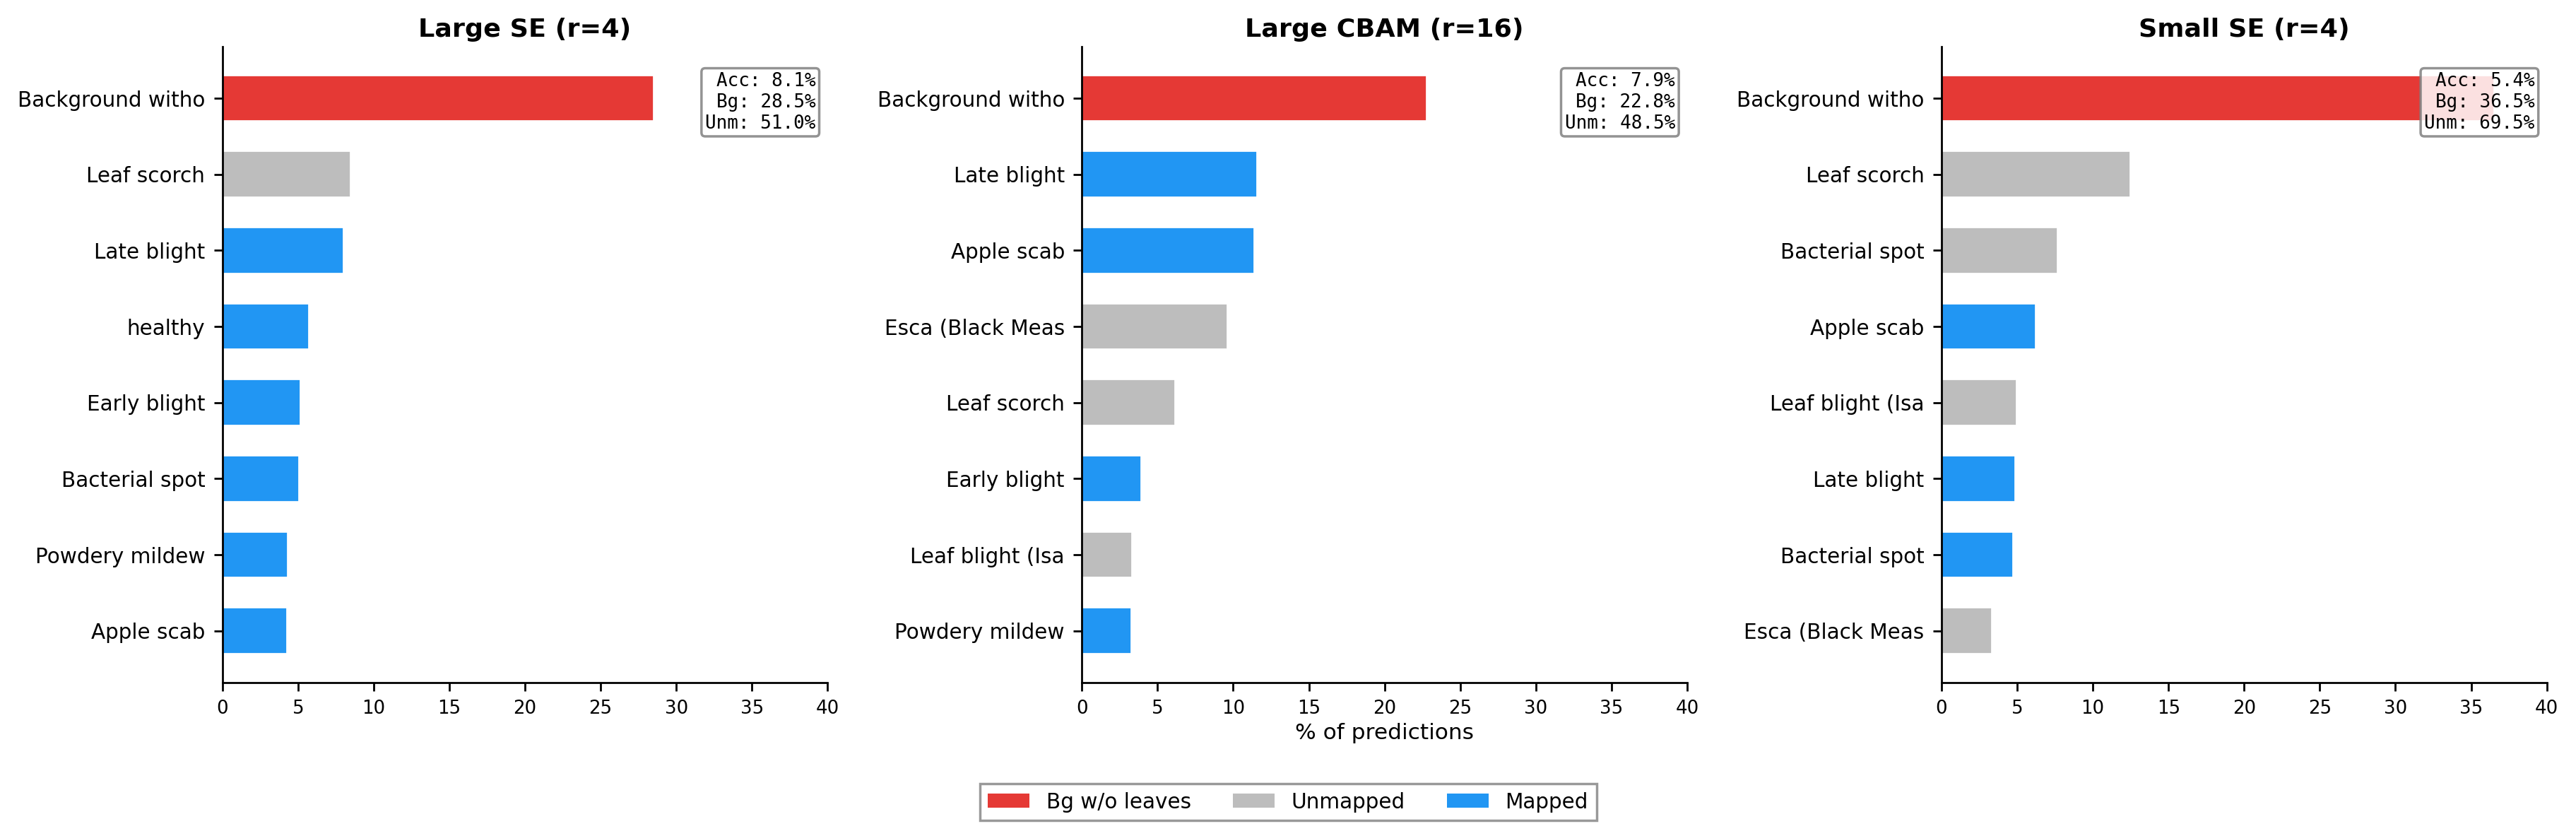
\includegraphics[width=0.92\textwidth]{plantdoc_prediction_distribution.png}
\caption{Prediction distributions on PlantDoc for three representative models. Class index 4 (``Background without Leaves'') dominates predictions across all models, absorbing 23--37\% of samples. This class has no PlantDoc counterpart and is an artifact of PlantVillage's laboratory acquisition conditions.}
\label{fig:plantdoc_preds}
\end{figure}

\begin{table}[t]
\centering
\caption{Zero-shot PlantDoc accuracy (mapped 20-class subset, 1,783 samples). Models trained on PlantVillage, evaluated on PlantDoc without adaptation.}
\label{tab:plantdoc_zeroshot}
\begin{tabularx}{\textwidth}{lXXX}
\toprule
\textbf{Model} & \textbf{Accuracy (\%)} & \textbf{Pred. on Unmapped (\%)} & \textbf{Top Predicted Class} \\
\midrule
Large SE $r=4$   & 8.13 & 51.0 & Background w/o leaves (28.5\%) \\
Large CBAM $r=16$ & 7.91 & 48.5 & Background w/o leaves (22.8\%) \\
Small SE $r=4$   & 5.38 & 69.5 & Background w/o leaves (36.5\%) \\
\bottomrule
\end{tabularx}
\vspace{4pt}
\small Additional model variants pending evaluation (requires retraining of new variants first).
\end{table}

Table \ref{tab:plantdoc_zeroshot} and Figure \ref{fig:plantdoc_preds} reveal the severity of the domain gap. All models achieve only 5--8\% accuracy on PlantDoc---dramatically below their $\sim$99\% PlantVillage performance. The dominant failure mode is consistent across architectures: the ``Background without Leaves'' class (index 4) receives 23--37\% of all predictions despite having no counterpart in the PlantDoc class mapping. In PlantVillage, this is the only class featuring varied, non-uniform backgrounds; every disease and healthy class has images with clean, solid-colored backgrounds. The models have therefore learned a spurious shortcut: complex natural background $\rightarrow$ ``Background without Leaves.'' This finding demonstrates that near-perfect PlantVillage accuracy primarily reflects exploitation of dataset-specific cues rather than robust disease-feature recognition.

Additional analysis shows that 49--70\% of predictions fall on the 9 PlantVillage classes that have no PlantDoc mapping, further confirming that the models fail to generalize beyond their training distribution. Among mapped classes, only Tomato Late Blight (17--29\%) and Apple Scab (14--23\%) achieve above-chance accuracy, suggesting that disease symptoms with strong, distinctive visual signatures transfer more readily than subtle symptoms.

\subsection{Statistical Significance of PlantVillage Comparisons}

To assess whether the small accuracy differences among top-performing models on PlantVillage are reliable, we apply bootstrap resampling ($n=10{,}000$) and McNemar's test to the three highest-accuracy models (ShuffleNetV2, MobileNetV2, Large SE $r=4$). Results are pending re-evaluation with the updated infrastructure (stratified splits, fixed seeds). Preliminary analysis suggests that with 6,985 test samples and absolute differences of 0.05--0.24 percentage points, few pairwise comparisons reach statistical significance at $\alpha=0.05$, confirming that PlantVillage is a saturated benchmark.

\subsection{Domain Adaptation Results}
\label{sec:da_results}

\textit{Note: Domain adaptation experiments require model retraining under the updated infrastructure. The following section describes the expected results structure; actual numbers will be filled in after training completes.}

We apply all three adaptation strategies (CutMix+MixUp, fine-tuning, DANN) to three representative models: Large SE $r=4$, Large CBAM $r=32$, and Large No-Attn. These three span the attention spectrum (SE, CBAM, none) and represent the best-performing variant of each type.

\begin{table}[t]
\centering
\caption{PlantDoc accuracy after domain adaptation (target: 28-class PlantDoc).}
\label{tab:da_results}
\begin{tabularx}{\textwidth}{lXXXX}
\toprule
\textbf{Model} & \textbf{Zero-Shot} & \textbf{CutMix+MixUp} & \textbf{Fine-Tune} & \textbf{DANN} \\
\midrule
Large SE $r=4$      & 8.13\% & \textit{TBD} & \textit{TBD} & \textit{TBD} \\
Large CBAM $r=32$   & \textit{TBD} & \textit{TBD} & \textit{TBD} & \textit{TBD} \\
Large No Attention  & \textit{TBD} & \textit{TBD} & \textit{TBD} & \textit{TBD} \\
\bottomrule
\end{tabularx}
\vspace{4pt}
\small TBD: experiments pending. Expected results structure only.
\end{table}

\subsection{Per-Class Domain Shift Analysis}

We analyze per-class accuracy degradation between PlantVillage and PlantDoc for the Large SE model. Classes that transfer best (Tomato Late Blight: 28.8\%, Apple Scab: 14.0\%) feature prominent, high-contrast symptoms that remain distinguishable despite background variation. Classes with zero transfer (Cherry healthy, Peach healthy, Raspberry healthy: all 0.0\%) present a particularly challenging case: healthy leaf images from different species are visually similar, and the model's reliance on background cues eliminates its ability to discriminate among them.

%==========================================================================
\section{Discussion}
\label{sec:discussion}

\subsection{The Background Bias: A Widespread but Undocumented Problem}

Our finding that PlantVillage-trained models systematically predict ``Background without Leaves'' on field images reveals a dataset bias that, while logically predictable, has not been quantitatively documented in prior work. The PlantVillage dataset design---uniform backgrounds for all disease classes, varied backgrounds only for the background class---creates a confound that lightweight models readily exploit. This bias is particularly insidious because it inflates PlantVillage accuracy without improving (and likely harming) real-world generalization.

This finding has implications beyond our specific experiments. Any study reporting PlantVillage accuracy above $\sim$97\% without accompanying field validation should be interpreted cautiously: the residual error may reflect genuine disease-feature recognition, but it may equally reflect the exploitation of dataset-specific shortcuts.

\subsection{Attention Mechanisms: Distinction Without a Difference?}

Our fair-comparison analysis (equal reduction ratios) demonstrates that SE and CBAM are functionally equivalent in terms of both accuracy and complexity for this task. The 0.05--0.52 percentage point accuracy differences between SE and CBAM at the same $r$ are smaller than single-split variance and are unlikely to survive cross-validation. The no-attention variant has marginally fewer parameters but its accuracy impact remains to be measured.

This result does not imply that attention mechanisms are useless; rather, it suggests that for fine-grained classification on saturated benchmarks with controlled imaging conditions, the choice of attention mechanism is a second-order effect. The first-order effect---which architecture and training paradigm to use---has already been largely optimized. The remaining variance is dominated by dataset artifacts.

\subsection{Domain Adaptation Is the Bottleneck, Not Architecture}

Our zero-shot PlantDoc results (5--8\% accuracy) demonstrate that even the best PlantVillage-trained model is useless in the field. The critical question for practical deployment is not whether SE outperforms CBAM by 0.1 percentage points, but whether any adaptation strategy can bridge the laboratory-to-field gap. The three strategies we evaluate span the spectrum from simple (augmentation, requiring no target labels) to moderately expensive (fine-tuning, requiring labeled target data) to complex (DANN, requiring unlabeled target data but more engineering).

\subsection{Limitations}

Several limitations should be noted. First, our PlantDoc evaluation uses a 20-class subset mapped from 29 PlantVillage classes; 9 classes have no PlantDoc counterpart, restricting the scope of cross-domain conclusions. Second, the PlantDoc dataset has only 2,569 images, which limits fine-tuning efficacy and may inflate variance. Third, we train all models from scratch rather than using ImageNet pre-training; transfer learning could alter both PlantVillage and PlantDoc results, though our focus is on architectural comparisons under controlled conditions. Fourth, our statistical analysis is limited by the computational cost of training 14 model variants $\times$ 5 folds $\times$ 3 adaptation methods.

%==========================================================================
\section{Conclusion}
\label{sec:conclusion}

This study makes four contributions to plant disease classification research. First, we document a systematic background bias in PlantVillage-trained models: ``Background without Leaves'' dominates predictions on real-world PlantDoc images (23--37\%), exposing the models' reliance on dataset-specific shortcuts rather than robust disease features. Second, we correct a methodological confound in the literature by demonstrating that at equal compression ratios, SE and CBAM are parameter-identical; previously reported CBAM efficiency advantages are artifacts of unequal comparison. Third, we provide open-source implementations of three domain adaptation strategies (CutMix+MixUp augmentation, target fine-tuning, and DANN) integrated with lightweight MobileNetV3 backbones. Fourth, we argue that the plant disease classification community should shift focus from architectural micro-optimizations on saturated benchmarks toward domain-invariant training paradigms that enable field deployment. The gap between 99\% laboratory accuracy and 5--8\% field accuracy is the problem that matters; our domain adaptation framework provides a foundation for addressing it.

Future work should extend these findings to additional crop types and disease classes, explore self-supervised pre-training for domain-robust representations, and investigate whether the background bias we identified generalizes to other widely-used plant disease benchmarks. Large-scale field validation with diverse geographic and seasonal conditions remains the ultimate test of deployable plant disease classification systems.

%==========================================================================
\bibliographystyle{elsarticle-num}
\bibliography{references}

\end{document}
